\chapter{Metric Improvements}

There are two general approaches for extracting simulation data into meaningful metrics: capture and report all raw data and use post processing to extract the metrics or capture only that data which we know to represent meaningful metrics and ignore the rest.  The first approach is valuable in that the volume of data has the potential to provide many first, second, and third order metrics which are not visible when sampling.  For example other researchers on this project are using trends in the data to help summarize the data at a higher level of abstraction.  Unfortunately the high volume of data also makes it more difficult to find meaningful metrics.  The sample approach simplifies the collection of specific metrics, however, this may make it more difficult to compare multiple metrics if the raw data which connects those metrics was not captured.    

 , extract trends in raw data to summarize the data at higher levels of abstraction, and sampling raw data at key points.  The first approach

The metrics presented in chapter 3 were obtained using the sampling approach.  The problem with this ad-hoc approach is that it creates disjoint data sets making it difficult to compare different metrics side by side in a timeline.  It also makes it difficult to verify that the metrics are accurate in relation to one another and the model.

To address these issues two different approaches are now being taken.  Other researchers are implementing the second of the previously mentioned approaches while for this thesis we present a combination of the first and third approaches.  Figure~\ref{fig:metric_gathering} shows the first in last out approach which is used to obtain more accurate metric data from the LSTS hierarchy.  For each time step in the simulation the Simulator will ask the Team for metrics which triggers the metric stack seen in figure~\ref{fig:metric_gathering}.  When it is time for a component to sample the raw data it will select a sample of the raw data and pass it to its parent.  The parent then selects its own sample data from the available raw data and the sample returned by its child.  This allows the component to perform pre-processing on the raw data which is much easier to accomplish while the data is still within the original context.  It also captures a unified timeline for all of the metrics.  We can see this in action by examining the Actor metric stack.  The Actor knows how many input channels he can listen on, his current state, etc\ldots  The Actor does not directly know what transitions are enabled, how many inputs are in those transitions, etc\ldots  Instead of trying to calculate all of this with multiple queries into the state the Actor simply asks the State object for its metrics.  The State then obtains/calculates metric values, obtaining metrics from sub-components if needed, before passing these values back to the Actor.  Once each Actor has returned a set of metrics the Team will then return these metrics, in the form of an array, to the Simulator for storage, post processing, and user display.  Results presented in the next chapter show the value of presenting the metrics in a unified timeline.

\begin{figure}[h]
\begin{center}
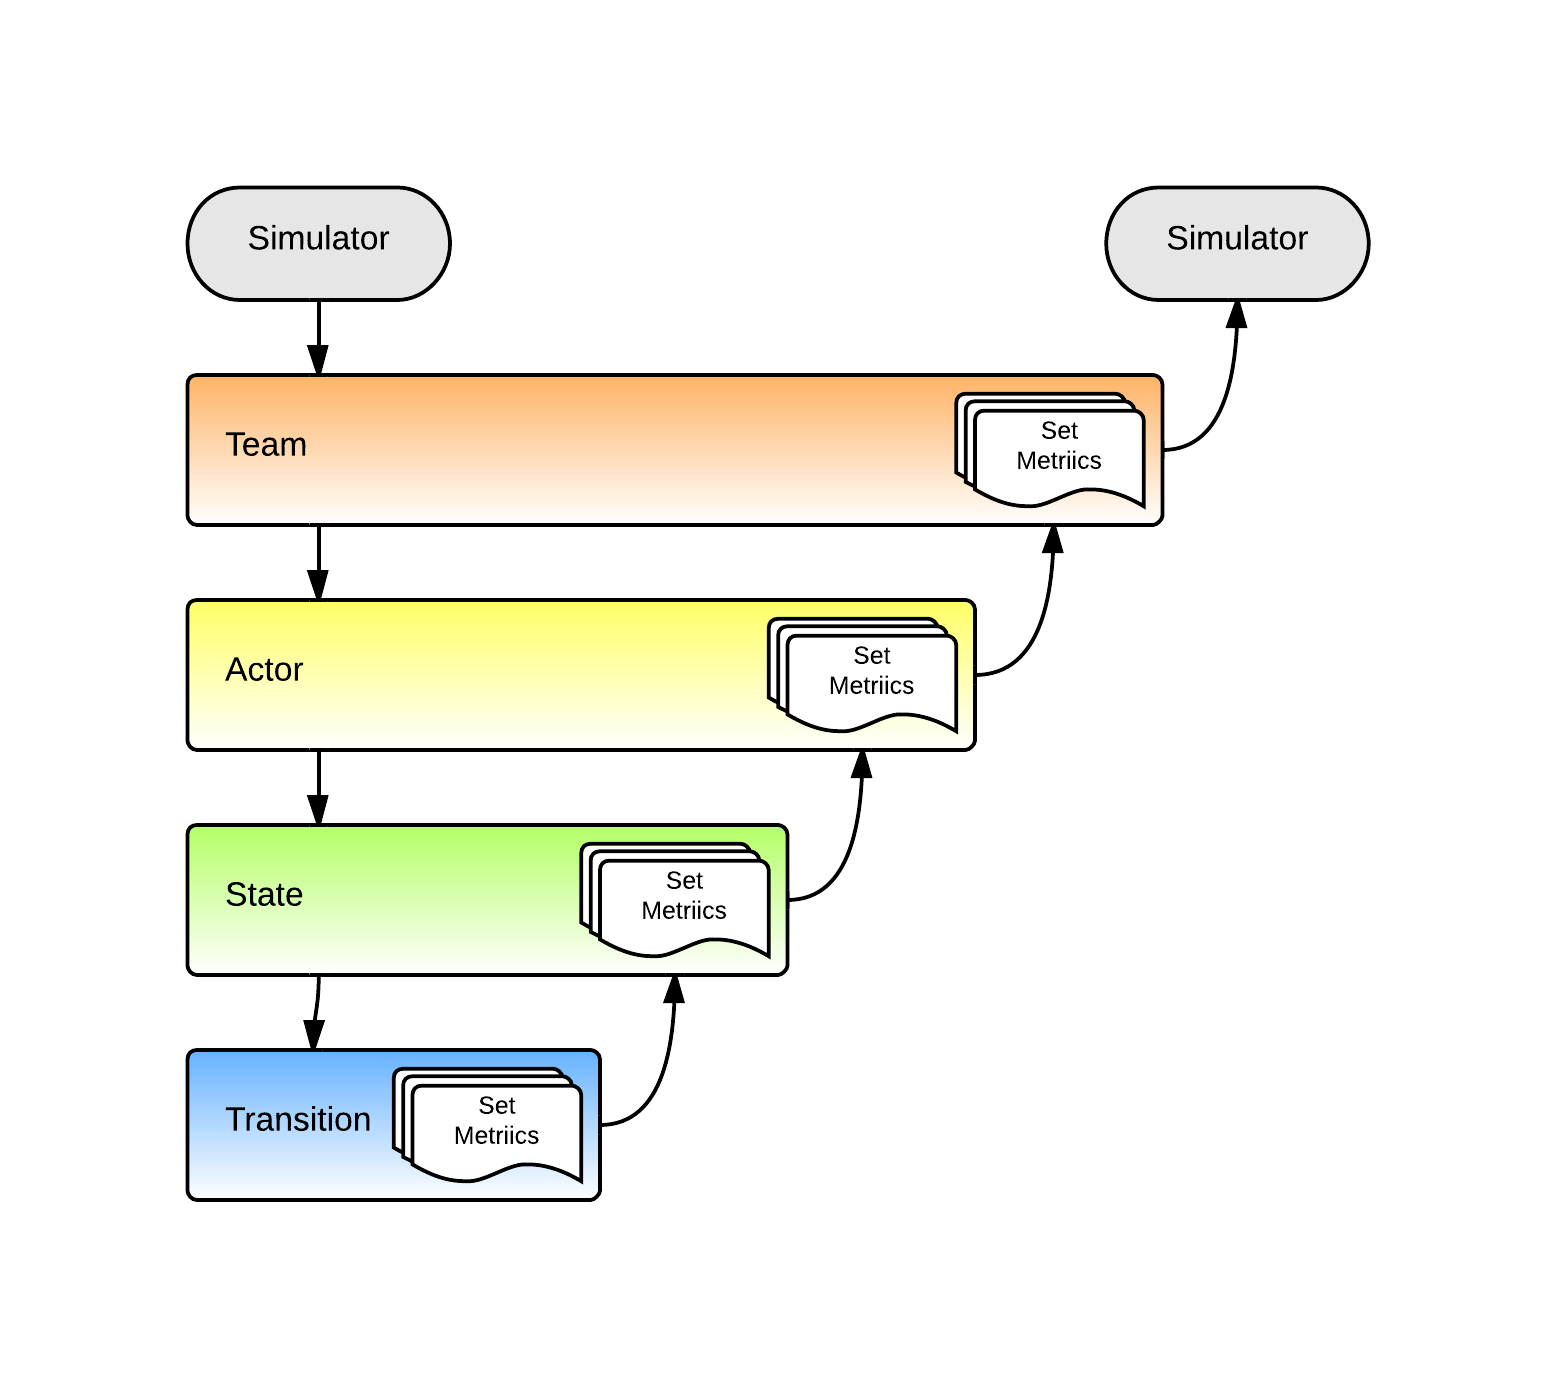
\includegraphics[width=6in]{metric_gathering.png}
\caption{Metric Gathering}
\label{fig:metric_gathering}
\end{center}
\end{figure}

\section{Wickens Workload Model}

Given the ability to extract Gathering the raw values from the model was the easy part.  The harder part is to take these raw values and convert them into a value which reflects Actor workload.  Since our model relies on Wickens Multiple Resource Theory~\cite{wickens2002multiple}.  We decided to try and replicate the simple computational model for predicting workload presented with the theory.  Wickens computational model takes the task difficulty, ranging from 0 to 2 where 0 is automated and 2 is difficult, of two tasks and adds them together.  He then adds the number of dimensional conflicts between the tasks, max of 4, which gives a result between 0 and 8~\cite{wickens2002multiple}.
	The difficulty of applying this model to our metrics is that we have removed the concept of tasks and replaced it with the notion of state.  In order to replicate Wickens computational model we needed a way to represent task difficulty (resource demand) in a similar fashion.  We first looked at transition duration.  The longer a task takes the more difficult it is.  While this might work it prevents the modeler from placing an Actor into a long running simple task which we feel would degrade the usefulness of this framework.  Next we looked at resources.  The problem is that our modeling framework only tracks what resources are being used and when.  Good for finding conflicts but not for determining how much load those resources are under.  It is possible that Wickens ran into the same problem because his simple computational model relies on the modelers experience and intuition to set the task difficulty, which is likely more accurate than implicitly constructing task difficulty based on resource consumption.  This led to the realization that we had no good way of explicitly defining an Actors task difficulty.  To address this we defined a new term called Actor load.  
	
\section{Actor Load}
Actor load represents an abstraction of the load an Actor is under for any given state.  Similar to Wickens model we will use values from 0-4.  Each Actor state will define its own load.  A load of 0 represents little to no load on the actor.  These are automated or transitional states.  A load of 4 represents simultaneously performing multiple high difficulty tasks.  Any value between 1 and 3 is some combination of task difficulty and the number of tasks being performed.

\section{Applying Wickens Computational Model}
By placing Actor Load into the State portion of our models we can now replicate the simple computational model Wickens used in his measurements.  Using the State load as the task difficulty the next step is to find the dimensionality of the resource conflicts.  Since a state represents 1 or more tasks this also presents a challenge.  To best approximate Wickens model we needed metrics which could represent one or more tasks.  We accomplish this by making the assumption that if an Actor has input from multiple sources in a state then multiple tasks are being performed.  It should be noted that we check the input channels for each transition in the current state but only the outputs of the current transition.  With these assumptions we are now ready to calculate dimensional conflicts, Figure~\ref{fig:multipleresourcetheory}.
For the Stage dimension (perception, cognition, response) we check to see if there are multiple sources of input or multiple targets for output.  If there are then we increment the dimensionality.   
For the Modality dimension (Audio, Visual) we check if there are more than a single active channel, input or output, of type audio or visual.  If there is then we increment the dimensionality.  
For the Focus dimension we check if there is more than one source for tactile outputs, if there are then we increment the dimensionality.  We do not check inputs as we have no way of distinguishing if a visual channel has focus.  This may need to be addressed in future work. 
For the Codes dimension (Spacial, Verbal) we check that the total number of audio inputs and outputs is greater than 1 or that the total number of visual inputs, visual outputs, and tactile outputs is greater than 1.  If either value is greater than 1 then we increment the dimensionality.  

By adding the task difficulty (state load) and the dimensionality together we obtain an adapted Wickens metric which we can then compare with our own metrics.

\begin{figure}[h]
\begin{center}
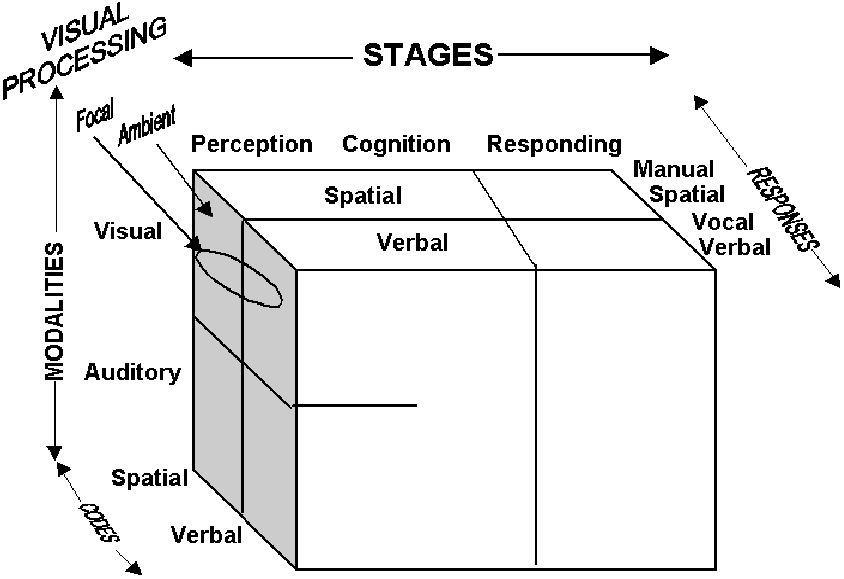
\includegraphics[width=6in]{multresourcetheory.png}
\caption{Multiple Resource Theory Dimensions}
\label{fig:multipleresourcetheory}
\end{center}
\end{figure}

\section{Changes to our Metrics}
For the resource workload category we now generate Actor metrics the following way.  Inputs are gathered from each transition that is part of the current state.  The outputs are collected from the active transition.  We also use the Actor load from the current state.  There are 2 main metrics the channel conflicts and the resource load.  Channel conflicts occur whenever more than one active channel share a type, such as multiple audio channels.  Since we currently only allow visual and audio input for human Actors this value ranges from 0 to 2.  The other metric is the resource load.  This metric attempts to quantify the load being placed on the Actors resources.  We break the resource load into two parts, input and output, the final result being the sum of both parts.  Each part is calculated by adding the number of active channels, number of layers read, number of memory objects read, and the number of active channel types.

For decision workload we have added input complexity and output complexity.  The input complexity is the total number of active inputs plus the number of memory inputs.  The output complexity is the number of output channels plus the number of memory outputs.  While there is overlap between these values and the resource workload metrics we leave it up to future work to analyze this relationship.  We have also modified the duration complexity metric.  Before adding Actor load we relied on the duration complexity to inform us of task difficulty.  We no longer apply the same weight to the durations.  Instead we are now using a logarithmic scale.  By assuming that durations are in seconds we classify any transition under a minute as 0 complexity and move up from there.  Our reasoning for this normalization is two fold.  First it is reasonable to assume that the more time a transition takes the more workload it requires, however, it is also reasonable to assume that there are diminishing returns associated with increasing the workload.  We would also like to compare the metrics together.  By normalizing this metric to a value between 0 and 6, for our model, we can show this metric side by side with the others.  


\subsection{Other Changes}
We also performed other refactorings to the modeling framework which facilitate the previously described changes and more.  As part of this re-factoring the connections to JPF were temporarily disabled in order to simplify the debugging process.  The results described in the next chapter were obtained by running the simulator as a stand alone application outside of JPF.  While this does prevent a deeper evaluation of the models state space the core model behavior still remains the same.  Unfortunately it prevented us from collecting the temporal workload metrics from the model.
